
%(BEGIN_QUESTION)
% Copyright 2006, Tony R. Kuphaldt, released under the Creative Commons Attribution License (v 1.0)
% This means you may do almost anything with this work of mine, so long as you give me proper credit

Et \textit{tank expert}-system bruker tre trykktransmittere for å måle nivå og tetthet av en væske i en stor lagertank.  De tre transmitterene er merket ``top'', ``middle'' og ``bottom'':

$$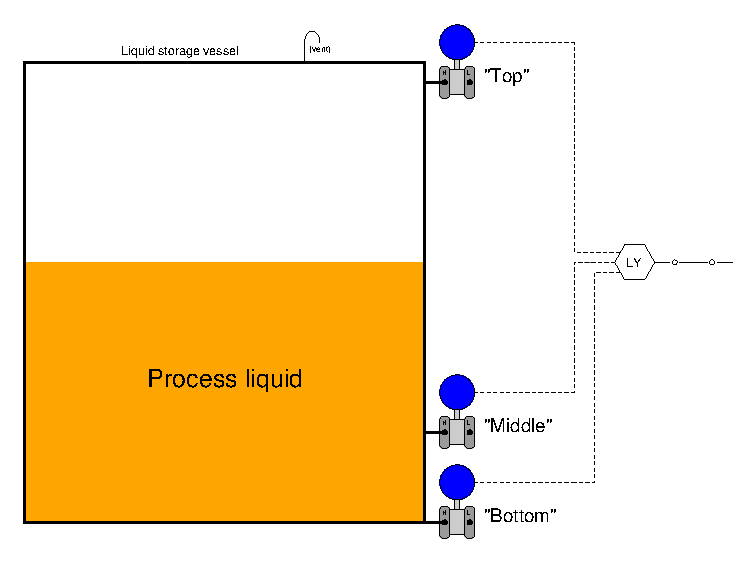
\includegraphics[width=15.5cm]{i00254x01.eps}$$

Tank expert-systemer bruker en datamaskin (LY i diagrammet) til å behandle data fra de tre trykktransmitterne og beregne både væsketetthet og væskenivå.  Avstanden mellom ``middle'' og ``bottom'' er kjent fra installasjon og lagt inn i datasystemet som en konstantverdi i beregningene.  Et viktig krav i et slikt system er at væskenivået må ligge over ``middle''-transmitteren for at tetthet skal kunne beregnes.

Anta at et tank expert-system har ``middle'' plassert 10 fot over tankbunnen, ``bottom'' helt i bunnen, og ``top'' helt i toppen.  Anta videre at tanken er ventilert i toppen (ingen damptrykksoppbygging), at høyden er 40 fot, og at væskenivået er 15 fot med spesifikk vekt 0.86.  Hvilke trykk vil de tre transmitterene rapportere til datasystemet under disse forholdene?  Med andre ord: hva blir ``rå'' inputdata til datasystemet?

\underbar{file i00254}
%(END_QUESTION)





%(BEGIN_ANSWER)

``Top'' pressure = 0 "W.C.

``Middle'' pressure = 51.6 "W.C.

``Bottom'' pressure = 154.8 "W.C.

%(END_ANSWER)





%(BEGIN_NOTES)


%INDEX% Measurement, level: hydrostatic pressure
%INDEX% Measurement, level: tank expert system

%(END_NOTES)
